\section{力的分解}
\subsection{基本原理}
力是矢量,力的加减满足平行四边形定则.力的合成的逆运算叫做力的分解.也就是\CJKunderwave{已知一个力求它的分力}的过程.

在这里有必要解释一下,研究力的分解的深刻含义:举一个例子,在小学大家刚开始学习算术的时候,老师教大家计算$13+27=?$,这可以先拆开再相加,则运算简洁快速不少,如下
$$13+27=10+3+20+7=10+20+(3+7)=40$$

力是一个矢量,则多个矢量相加,按平行四边形定则可行,但是具体运算要复杂的多,因为要画多个平行四边形,同时每个平行四边形都要使用余弦定理计算,涉及开方和三角函数运算.为了方便运算,往往需要采用先分解为两个相互垂直的方向的分力,然后再把每个坐标轴上的分力叠加起来,最后再使用勾股定理计算则可以简化许多---这个方法叫做正交分解法.

力的分解与力的合成不同,力的合成结果是唯一的,但是力的分解,是将一个力分解为二个力或多个力,这在数学上有无数种分解方式,就象$9=1+8=2+7=\cdots $一样.正是力的分解的这种任意性,结合实际情况可以将计算变的大为简化.根据实际情况,可以定出如下力的分解法:
\begin{enumerate}
  \item 根据\CJKunderwave{力的实际作用}效果定出两个分力的方向
  \item 根据\CJKunderwave{两个分力}的方向作出平行四边形
  \item 利用数学知识\CJKunderwave{解三角形},分析,计算分力的大小.
\end{enumerate}
\subsection{例题分析}
\begin{calculate}
 1.如<:
 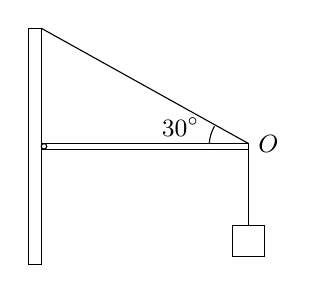
\begin{tikzpicture}
   \draw (-0.2,1.5) rectangle (-1pt,-1.5);
   \draw (0,0) circle [radius=1pt];
   \draw (-1pt,-1pt) rectangle (2.598,1pt) node [anchor=west]{\small $O$};
   \draw (-1pt,1.5) -- (2.598,1pt);
   \draw (2.598,1pt)--(2.598,-1);
   \draw (2.398,-1) rectangle (2.798,-1.4);
   \draw (2.165,0.254) arc (150:177:0.5);
   \draw (2.098,0) node [anchor=south east]{\small $30^\circ$};
 \end{tikzpicture}
 :>所示,轻杆与柱子之间用铰链连接,杆的末端吊着一个重为$30N$ 的物体,轻绳与水平轻杆之间的夹角为$\theta=30^\circ$ ,求轻绳和杆各受到多大的力?(结果保留两位有效数字)

 a.$60N$ \qquad $52N$

 e.物体静止则受力平衡,所以重力与竖直绳的拉力平衡,则竖直绳的拉力大小$F=G$.由于绳的拉力一定沿绳指向绳收缩的方向,铰链所受力的方向一定沿杆的方向.所以得出力分解的两个效果的方向就是绳收缩的方向和杆压缩的方向.由此作平行四边形如
 <:
 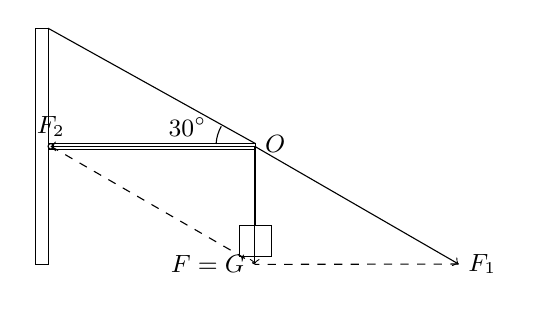
\begin{tikzpicture}
   \draw (-0.2,1.5) rectangle (-1pt,-1.5);
   \draw (0,0) circle [radius=1pt];
   \draw (-1pt,-1pt) rectangle (2.598,1pt) node [anchor=west]{\small $O$};
   \draw (-1pt,1.5) -- (2.598,1pt);
   \draw (2.598,1pt)--(2.598,-1);
   \draw (2.398,-1) rectangle (2.798,-1.4);
   \draw (2.165,0.254) arc (150:177:0.5);
   \draw (2.098,0) node [anchor=south east]{\small $30^\circ$};
   \draw [->](2.589,0)--(0,0) node [anchor=south]{\small $F_2$};
   \draw [->](2.589,0)--(2.589,-1.4948) node [anchor=east] {\small $F=G$};
   \draw [->](2.589,0)--(5.178,-1.4948) node [anchor=west] {\small $F_1$};
   \draw [dashed] (0,0)--(2.589,-1.4948);
   \draw [dashed] (5.178,-1.4948)--(2.589,-1.4989);
 \end{tikzpicture}
 :>所示,由几何关系得
 $$F_1=\cfrac{G}{\sin\theta}=60N,F_2=\cfrac{G}{\tan\theta}\approx 52N$$

 \end{calculate}

 \newpage

 \begin{selection}
 2.如<:
 \begin{tikzpicture}
   \draw (0,0) node [anchor=east] {\small O}--(3,0) node [anchor=north east] {\small $F_2$ 的方向};
   \draw [->,>=stealth] (0,0)--(2,1.5) node [anchor=east] {$F$};
   \draw (0.3,0) arc (0:37:0.3);
   \draw (30:0.3) node [anchor=west]{\small $\theta$};
 \end{tikzpicture}
 :>所示,将力$F$ (大小已知)分解为两个分力$F_1$ 和$F_2$ ,$F_2$ 和$F$ 的夹角$\theta$ 小于 $90^\circ$ ,则下列说法正确的是
 A.当$F_1>\sin\theta$ 时,肯定有两组解
 B.当 $F>F_1>F\sin\theta$ 时,肯定有两组解
 C.当$F_1<F\sin\theta$ 时,有唯一一组解
 D.当$F_1<F\sin\theta $ 时,无解.

 a.BD

 e.已知合力的大小、一个分力的方向,根据平行四边形定则(三角形定则更方便)作图,如
 <:
 \begin{tikzpicture}
   \draw (0,0) node [anchor=east] {\small O}--(5,0) node [anchor=north east] {\small $F_2$ 的方向};
   \draw [->,>=stealth] (0,0)--(2,1.5) node [anchor=east] {\small $F$};
   \draw (0.3,0) arc (0:37:0.3);
   \draw (30:0.3) node [anchor=west]{\small $\theta$};
   \draw  (2,0)--(2,1.5) node [anchor=west] {\small $F_1$};
   \draw  (1,0)--(2,1.5) node [anchor=west] {\small $F_1$};
   \draw  (2.5,0)--(2,1.5) node [anchor=west] {\small $F_1$};
   \draw  (4.5,0)--(2,1.5) node [anchor=west] {\small $F_1$};
   \draw (2,0) rectangle (2.2,0.2);
 \end{tikzpicture}
 :>所示
 \newline
 当$F>F_1>F\sin\theta$ , 一定有两组解
 \newline
 当 $F_1>F$ 时,有唯一一组解
 \newline
 当$F_1<F\sin\theta $ ,无解.
 
 \end{selection}

 \begin{calculate}
3.如<:
\begin{tikzpicture}
  \draw (0,0) rectangle (1,0.8);
  \draw [dashed] (0.5,0.4)--(1.5,0.4);
  \draw[->,>=stealth] (0.5,0.4) -- (1.5,0.97735) node [anchor=west] {\small $F$};
  \draw[pattern=north west lines] (-0.5,-0.2)--(-0.5,0)--(1.5,0)--(1.5,-0.2);
  \draw (0.8,0.4) arc (0:30:0.3);
  \draw (0.7,0.3) node [anchor=south west] {\tiny $\theta$};
\end{tikzpicture}
:>所示,水平面上有一重$60N$的物体,在与水平方向成$30^\circ$ 角斜向上,大小为$20N$的拉力作用下匀速运动,求地面对物体的支持力和摩擦力的大小.

a.$50N$ \quad $10\sqrt{3}N$

e.对物体进行受力分析,如<:
\begin{tikzpicture}
  \draw (0,0) rectangle (1,0.8);
  \draw [dashed] (0.5,0.4)--(1.5,0.4);
  \draw[->,>=stealth] (0.5,0.4) -- (1.5,0.97735) node [anchor=west] {\small $F$};
  \draw[pattern=north west lines] (-0.5,-0.2)--(-0.5,0)--(1.5,0)--(1.5,-0.2);
  \draw (0.8,0.4) arc (0:30:0.3);
  \draw (0.7,0.3) node [anchor=south west] {\tiny $\theta$};
  \draw [->,>=stealth] (-1,0.4)--(2,0.4) node [anchor=north]{\small $x$};
  \draw [->,>=stealth] (0.5,-1)--(0.5,2) node [anchor=west] {\small $y$};
  \draw [dashed](1.5,0.4)--(1.5,0.97735);
  \draw [->,>=stealth] (0.5,0.4)--(1.5,0.4) node [anchor=north] {\tiny $F_x$};
  \draw [dashed](0.5,0.97735) --(1.5,0.97735);
  \draw [->,>=stealth] (0.5,0.4)--(0.5,0.97735) node [anchor=east]{\tiny $F_y$};
  \draw [->,>=stealth] (0.5,0.4)--(0.5,1.5) node [anchor=east] {\tiny $F_N$};
  \draw [->,>=stealth] (0.5,0.4)--(-0.5,0.4) node [anchor=north] {\tiny $F_f$};
\end{tikzpicture}
:>所示,物体受重力$G$,支持力$F_N$,拉力$F$,摩擦力$F_f$.建立正交直角坐标系,对力$F$ 进行正交分解得两个分力的大小分别为
$$F_x=F\cos\theta,F_y=F\sin\theta$$
$y$方向受力平衡:
$$F_N+F\sin30^\circ -G=0$$
$x$方向受力平衡:
$$F_f-F\cos30^\circ =0$$
以上两式联立解得:
$$F_N=50N,F_f=10\sqrt{3}N$$

ee.注意:在使用正交分解法时,坐标系的建立原则上是任意的,它都能解决问题.但是实际使用时,要兼顾计算的简洁,如果将坐标轴建立在相互垂直的力上,且使尽量多的力落在坐标轴上,那么需要分解的力就少了,这样就能减少计算量.比如这里,支持力$F_N$和摩擦力$F_f$相互垂直,则按这个规则建立坐标轴后,只有拉力$F$ 需要分解,这样计算量就减少了.同学们在使用时要仔细研究分析之后选择最简单的建立坐标系的才能不断提高解题能力.

\end{calculate}
\begin{selection}
4.如<:
\begin{tikzpicture}
  \draw (1,0) node [anchor= south west] {\tiny $D$} arc (0:180:1);
  \draw [pattern=north west lines] (-1.5,-0.2)--(-1.5,0)--(-0.5,0)--(-0.5,-0.2);
  \draw [pattern=north west lines] (1.5,-0.2)--(1.5,0)--(0.5,0)--(0.5,-0.2);
  \draw [dashed] (-1,0)--(1,0);
  \draw (0,0) node [anchor=north] {\tiny $O$}-- (135:1) node [anchor=south east] {\tiny $B$};
  \draw (0,0) --(45:1) node [anchor=south west] {\tiny $A$};
  \draw (0,0) -- (0,-1);
  \draw (-0.2,-1) rectangle (0.2,-1.4);
  \draw (0,-1.2) node {\tiny $M$};
  \draw [dashed] (0,0)--(0,1) node [anchor=south] {\tiny $C$};
\end{tikzpicture}
:>所示,质量为$M$ 的物体用$OA$ 和$OB$ 两根等长的绳子悬挂在半弧形的支架上,$B$ 点固定不动,$A$ 点则由顶点$C$ 沿圆弧向$D$ 移动.在此过程中,绳子$OA$ 的张力将
A.由大变小
B.由小变大
C.先减小再增大
D.先增大再减小

a.C

e.此题目画三角形更方便一些.如<:
\begin{tikzpicture}
  \draw (1,0) node [anchor= south west] {\tiny $D$} arc (0:180:1);
  \draw [pattern=north west lines] (-1.5,-0.2)--(-1.5,0)--(-0.5,0)--(-0.5,-0.2);
  \draw [pattern=north west lines] (1.5,-0.2)--(1.5,0)--(0.5,0)--(0.5,-0.2);
  \draw [dashed] (-1,0)--(1,0);
  \draw (0,0) node [anchor=north] {\tiny $O$}-- (135:1) node [anchor=south east] {\tiny $B$};
  \draw (0,0) --(45:1) node [anchor=south west] {\tiny $A$};
  \draw (0,0) -- (0,-1);
  \draw (-0.2,-1) rectangle (0.2,-1.4);
  \draw (0,-1.2) node {\tiny $M$};
  \draw [dashed] (0,0)--(0,1) node [anchor=south] {\tiny $C$};
  \draw [->,>=stealth] (0,0)--(0,-2) node [anchor=north east] {\tiny $Mg$};
  \draw [<-,>=stealth] (0,0) -- (315:2);
  \draw [->,>=stealth] (0,-2) -- +(45:1.414) node [anchor=south west]{\tiny 1};
  \draw [->,>=stealth] (0,-2)-- (0.7071,-0.7071) node [anchor=south west]{\tiny 2};
  \draw [->,>=stealth] (0,-2)-- (1.414,-1.414) node [anchor=south west]{\tiny 3};
  \draw (0,-0.3) arc (270:315:0.3);
  \draw (270:0.2) node [anchor=north west]{\tiny $\theta$};
\end{tikzpicture}
:>所示,画出了三种情况力的三角形,当$OA$ 的力在 1位置时,$F_A$ 与 $F_B$ 垂直,此时$F_A=Mg\sin\theta$ 是最小的.当 $OA$ 的力 在2或者 3位置时,$F_A>Mg\sin\theta$,所以绳子 $OA$ 的张力先减小再增大.
\newline
同学们注意:在力的动态变化分析时,一般会是三个力,已知一个力的大小和方向,第二个力的方向,问第三个力的情况.这时候画力的三角形要比平行四边形简单的多.如果物体的受力个数超过三个,则应当据正交分解法求出所讨论的力的大小与角度的关系,然后据函数的增减性来判断,会更加清析一些.

\end{selection}
\newpage
\begin{selection}
  
1.(多选)如<:
\begin{tikzpicture}
  \draw [pattern=north west lines] (-1.5,-0.2)--(-1.5,0)--(1.5,0)--(1.5,-0.2);
  \draw (-1,0) -- (1,0) -- (1,1.5) -- (-1,0)--cycle;
  \draw [rotate around={37:(-1,0)}] (0.4,0) rectangle (0.8,0.4);
  \draw [->,>=stealth,rotate around={37:(-1,0)}] (0.6,0.2) -- + (-127:1) node [anchor=west] {\small $mg$};
  \draw [->,>=stealth,rotate around={37:(-1,0)}] (0.6,0.2) -- + (-0.60182,0) node [anchor=east] {\small $F_1$};
  \draw [->,>=stealth,rotate around={37:(-1,0)}] (0.6,0.2) -- + (0,-0.79864) node [anchor=west] {\small $F_2$};
  \draw [dashed,rotate around={37:(-1,0)}] (-0.00182,-0.59864) -- (0.6,-0.59864);
  \draw [dashed,rotate around={37:(-1,0)}] (-0.00182,-0.59864) -- (-0.00182,0.2);
  \draw [->,>=stealth,rotate around={37:(-1,0)}] (0.6,0.2) -- (0.6,1) node [anchor=east] {\small $F_N$}; 
\end{tikzpicture}
:>所示,光滑斜面上物体重力$mg$ 分解为$F_1$ 和$F_2$ 两个力,下列说法正确的是
A.物体受到重力$mg$ , $F_N$ , $F_1$ ,$F_2$ 四个力作用
B.物体只受到重力$mg$ 和斜面的支持力$F_N$ 的作用
C.$F_1$ 是斜面作用在物体上使物体下滑的力,$F_2$ 是物体对斜面的压力
D.力$F_N$ ,$F_1$,$F_2$ 三力的作用效果与力$mg$ ,$F_N$ 两个力的作用效果相同

a.BD

e.由重力的作用效果分析,再由力产生的原因进行判断$F_1$ 和$F_2$ 两个力是重力$mg$ 的两个分力,其作用效果与重力$mg$ 等效,所以$F_2$ 不是物体对斜面的压力,物体只受重力$mg$ 和斜面的支持力$F_N$ 的作用,故 B,D正确.

\end{selection}
\begin{calculate}
  1. 如 
  <:
\begin{tikzpicture}
  \draw[pattern=north west lines] (-0.5,1.7)--(-0.5,1.5)--(0.5,1.5)--(0.5,1.7);
  \draw (0,0.2)--(0,1.5);
  \draw (0,0) circle [radius=2mm];
  \draw (0,-0.5) node [anchor=north] {\small 甲};
\end{tikzpicture}
  \qquad
\begin{tikzpicture}
  \draw (-1,0)--(-0.5,0);
  \draw (-0.5,0) arc (180:360:0.5);
  \filldraw[black] (0,0) node [anchor=south] {\small $O$} circle [radius=1pt];
  \draw (0.5,0)--(1,0);
  \draw[black,rotate around={26.5:(-0.3,-0.4)}] (-0.3,-0.4) rectangle (1,-0.3) node [anchor=west] {\small $P$};
  \draw (-0.3,-0.4) node [anchor=north east] {\small $A$};
  \draw (0.5,0) node [anchor=north west] {\small $B$};
  \draw (0,-1.5) node [anchor=north] {\small 乙};
\end{tikzpicture}
  \qquad
\begin{tikzpicture}
 \draw (30:2)--(210:0.5)--+(2.2,0); 
 \draw (60:1.2) circle [radius=0.6];
 \filldraw [black] (60:1.2) circle [radius=1pt];
 \filldraw [black,rotate around={-90:(0,0)}](0,0) rectangle (-1.5,-0.1);
  \draw (0.7,-0.5) node [anchor=north] {\small 丙};
\end{tikzpicture}
  \qquad
\begin{tikzpicture}
  \draw [pattern=north west lines] (-1,-0.2)--(-1,0)--(1,0)--(1,-0.2); 
  \draw (0,0.5) circle [radius=0.5];
  \filldraw[black] (0,0.5) circle [radius=1pt];
  \draw (-0.7,0.5) node {\small $P$};
  \draw [->,>=stealth] (-0.8,1.5) -- (0.8,1.5) node [anchor=west] {\small v};
  \draw (0,-0.5) node [anchor=north] {\small 丁};
\end{tikzpicture}
  :>
所示,对物体$P$ 作受力分析,其中甲、乙、丙中物体$P$ 处于静止状态,丁中物体$P$ 在水平面上匀速滚动.

e.对各物体受力分析如
<:
\begin{tikzpicture}
  \draw[pattern=north west lines] (-0.5,1.7)--(-0.5,1.5)--(0.5,1.5)--(0.5,1.7);
  \draw (0,0.2)--(0,1.5);
  \draw (0,0) circle [radius=2mm];
  \filldraw[black] (0,0) circle [radius=1pt];
  \draw (0,-0.5) node [anchor=north] {\small 甲};
  \draw [->,>=stealth](0,0) --(0,-1) node [anchor=west] {\small $mg$};
  \draw [->,>=stealth](0,0) --(0,1) node [anchor=west] {\small $T$};
\end{tikzpicture}
  \qquad
\begin{tikzpicture}
  \draw (-1,0)--(-0.5,0);
  \draw (-0.5,0) arc (180:360:0.5);
  \filldraw[black] (0,0) node [anchor=south] {\small $O$} circle [radius=1pt];
  \draw (0.5,0)--(1,0);
  \draw[black,rotate around={26.5:(-0.3,-0.4)}] (-0.3,-0.4) rectangle (1,-0.3) node [anchor=west] {\small $P$};
  \draw (-0.3,-0.4) node [anchor=north east] {\small $A$};
  \draw (0.5,0) node [anchor=north west] {\small $B$};
  \draw (0,-1.5) node [anchor=north] {\small 乙};
  \draw[->,>=stealth] (-0.3,-0.4) --(0,0) node [anchor=east] {\small $F_A$};
  \draw[->,>=stealth] (0.5,0) --+(116.5:0.5) node [anchor=west] {\small $F_B$};
  \draw[->,>=stealth] (0.2817,-0.06)--+(0,-1) node [anchor=west] {\small $mg$};
\end{tikzpicture}
  \qquad
\begin{tikzpicture}
 \draw (30:2)--(210:0.5)--+(2.2,0); 
 \draw (60:1.2) circle [radius=0.6];
 \filldraw[black] (60:1.2) circle [radius=1pt];
 \filldraw [black,rotate around={-90:(0,0)}](0,0) rectangle (-1.5,-0.1);
  \draw (0.7,-0.5) node [anchor=north] {\small 丙};
  \draw[->,>=stealth] (60:1.2) -- +(0,-1) node [anchor=west] {\small $mg$};
  \draw[->,>=stealth] (60:1.2) -- +(1,0) node [anchor=west] {\small $F_{N1}$};
  \draw[->,>=stealth] (60:1.2) -- +(-0.5,0.816) node [anchor=west] {\small $F_{N2}$};
\end{tikzpicture}
  \qquad
\begin{tikzpicture}
  \draw [pattern=north west lines] (-1,-0.2)--(-1,0)--(1,0)--(1,-0.2); 
  \draw (0,0.5) circle [radius=0.5];
  \filldraw[black] (0,0.5) circle [radius=1pt];
  \draw (-0.7,0.5) node {\small $P$};
  \draw [->,>=stealth] (-0.8,1.5) -- (0.8,1.5) node [anchor=west] {\small v};
  \draw (0,-0.5) node [anchor=north] {\small 丁};
  \draw[->,>=stealth] (0,0.5) -- (0,-0.5) node [anchor=west] {\small $mg$};
  \draw[->,>=stealth] (0,0.5) -- (0,1.5) node [anchor=west] {\small $F_N$};
\end{tikzpicture}
:>所示.

2.如<:
\begin{tikzpicture}
  \draw (-0.5,0.5) circle [radius=0.5]; 
  \draw (0.4,0.4) node {\small A} circle [radius=0.4];
  \draw [color=white,pattern=north west lines] (-1.1,-0.2)--(-1.1,0)--(1,0)--(1,-0.2);
  \draw (-1.1,0)--(1,0);
\end{tikzpicture}
\qquad
\begin{tikzpicture}
  \draw (0,0.7) node {\small A} circle [radius=0.6]; 
  \draw [color=white,pattern=north west lines] (-1,-0.2)--(-1,0)--(1,0)--(1,-0.2);
  \draw (-1,0)--(1,0);
  \draw (0,0.7)++(240:0.6)--+(150:0.6);
  \draw (0,0.7)++(240:0.6)--+(330:0.4);
  \draw (0,0.7)++(330:0.6)--+(60:0.5);
  \draw (0,0.7)++(330:0.6)--+(240:0.45);
\end{tikzpicture}
\qquad
\begin{tikzpicture}
  \draw [color=white,pattern=north west lines] (-1,-0.2)--(-1,0)--(1,0)--(1,-0.2);
  \draw (-1,0)--(1,0);
  \draw (-0.5,0)--(0.9,0.7)--(0.9,0);
  \draw (-0.1,0.2)++(120:0.1) node [anchor=east] {\small A} circle [radius=0.1];
  \draw (-0.1,0.2)++(120:0.1)++(45:0.1)--+(45:1);
  \draw (-0.1,0.2)++(120:0.1)++(45:0.1)++(45:1)--+(0.4,0);
  \draw (-0.1,0.2)++(120:0.1)++(45:0.1)++(45:1)--+(-1.4,0);
\end{tikzpicture}
\qquad
\begin{tikzpicture}
  \draw [color=white,pattern=north west lines] (-1,-0.2)--(-1,0)--(1,0)--(1,-0.2);
  \draw (-1,0)--(1,0);
  \draw (-0.5,0)--(0.9,0.7)--(0.9,0);
  \draw (-0.1,0.2)++(120:0.1) node [anchor=east] {\small A} circle [radius=0.1];
  \draw (-0.1,0.2)++(120:0.1)++(0,0.1)--+(0,0.65);
  \draw (-0.1,0.2)++(120:0.1)++(0,0.1)++(0,0.65)--+(1.1,0);
  \draw (-0.1,0.2)++(120:0.1)++(0,0.1)++(0,0.65)--+(-0.9,0);
\end{tikzpicture}
:>所示,物体A均处于静止状态,且接触面光滑,请画出物体A的受力分析图.


e.各物体受力分析如下
<:
\begin{tikzpicture}
  \draw (-0.5,0.5) circle [radius=0.5]; 
  \draw (0.4,0.4) node [anchor=west] {\small A} circle [radius=0.4];
  \draw [color=white,pattern=north west lines] (-1.1,-0.2)--(-1.1,0)--(1,0)--(1,-0.2);
  \draw (-1.1,0)--(1,0);
  \draw [->,>=stealth] (0.4,0.4) --+(0,-1) node [anchor=east] {\small $mg$};
  \draw [->,>=stealth] (0.4,0.4) --+(0,1) node [anchor=east] {\small $F_N$};
  \filldraw (0.4,0.4) circle [radius=1pt];
\end{tikzpicture}
\qquad
\begin{tikzpicture}
  \draw (0,0.7) node [anchor=east] {\small A} circle [radius=0.6]; 
  \draw [color=white,pattern=north west lines] (-1,-0.2)--(-1,0)--(1,0)--(1,-0.2);
  \draw (-1,0)--(1,0);
  \draw (0,0.7)++(240:0.6)--+(150:0.6);
  \draw (0,0.7)++(240:0.6)--+(330:0.4);
  \draw (0,0.7)++(330:0.6)--+(60:0.5);
  \draw (0,0.7)++(330:0.6)--+(240:0.45);
  \filldraw (0,0.7) circle [radius=1pt];
  \draw [->,>=stealth] (0,0.7)--+(0,-1.4) node [anchor=west] {\small $mg$};
  \draw [->,>=stealth] (0,0.7)--+(150:1) node [anchor=west] {\small $F_{N1}$};
  \draw [->,>=stealth] (0,0.7)--+(60:1) node [anchor=west] {\small $F_{N1}$};
  \draw [dashed](0,0.7)--++(240:0.6);
  \draw [dashed](0,0.7)--++(330:0.6);
\end{tikzpicture}
\qquad
\begin{tikzpicture}
  \draw [color=white,pattern=north west lines] (-1,-0.2)--(-1,0)--(1,0)--(1,-0.2);
  \draw (-1,0)--(1,0);
  \draw (-0.5,0)--(0.9,0.7)--(0.9,0);
  \draw (-0.1,0.2)++(120:0.1) node [anchor=east] {\small A} circle [radius=0.1];
  \draw (-0.1,0.2)++(120:0.1)++(45:0.1)--+(45:1);
  \draw (-0.1,0.2)++(120:0.1)++(45:0.1)++(45:1)--+(0.4,0);
  \draw (-0.1,0.2)++(120:0.1)++(45:0.1)++(45:1)--+(-1.4,0);
  \filldraw (-0.1,0.2)++(120:0.1) circle [radius=1pt];
  \draw [->,>=stealth] (-0.1,0.2)++(120:0.1)--+(0,-1) node [anchor=east] {\small $mg$}; 
  \draw [->,>=stealth] (-0.1,0.2)++(120:0.1)--+(135:0.8) node [anchor=west] {\small $F_N$};
  \draw [->,>=stealth] (-0.1,0.2)++(120:0.1)--+(45:0.7) node [anchor=west] {\small $F_T$};
\end{tikzpicture}
\qquad
\begin{tikzpicture}
  \draw [color=white,pattern=north west lines] (-1,-0.2)--(-1,0)--(1,0)--(1,-0.2);
  \draw (-1,0)--(1,0);
  \draw (-0.5,0)--(0.9,0.7)--(0.9,0);
  \draw (-0.1,0.2)++(120:0.1) node [anchor=east] {\small A} circle [radius=0.1];
  \draw (-0.1,0.2)++(120:0.1)++(0,0.1)--+(0,0.65);
  \draw (-0.1,0.2)++(120:0.1)++(0,0.1)++(0,0.65)--+(1.1,0);
  \draw (-0.1,0.2)++(120:0.1)++(0,0.1)++(0,0.65)--+(-0.9,0);
  \filldraw (-0.1,0.2)++(120:0.1)  circle [radius=1pt];
  \draw [->,>=stealth] (-0.1,0.2)++(120:0.1) --+(0,-1) node [anchor=west] {\small $mg$};
  \draw [->,>=stealth] (-0.1,0.2)++(120:0.1) --+(0,1) node [anchor=west] {\small $F_T$};
\end{tikzpicture}
:>所示.

8.如<:
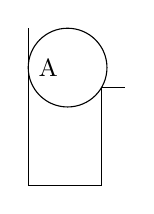
\begin{tikzpicture}
  \draw (0,1.5) node [anchor=east] {\small A} circle [radius=0.5];
  \draw (0,1.5)++(330:0.5)--+(0.3,0);
  \draw (0,1.5)++(330:0.5)--++(0,-1.25)--++(-0.933,0)--++(0,2);
\end{tikzpicture}
:>所示 ,画出物体A所受到的弹力示意图.

\end{calculate}
